\begin{center}
  \Large
  \textbf{BIOGRAFI PENULIS}
\end{center}

\addcontentsline{toc}{chapter}{BIOGRAFI PENULIS}

\vspace{2ex}

\begin{wrapfigure}{L}{0.3\textwidth}
  \centering
  \vspace{-3ex}
  % Ubah file gambar berikut dengan file foto dari mahasiswa
  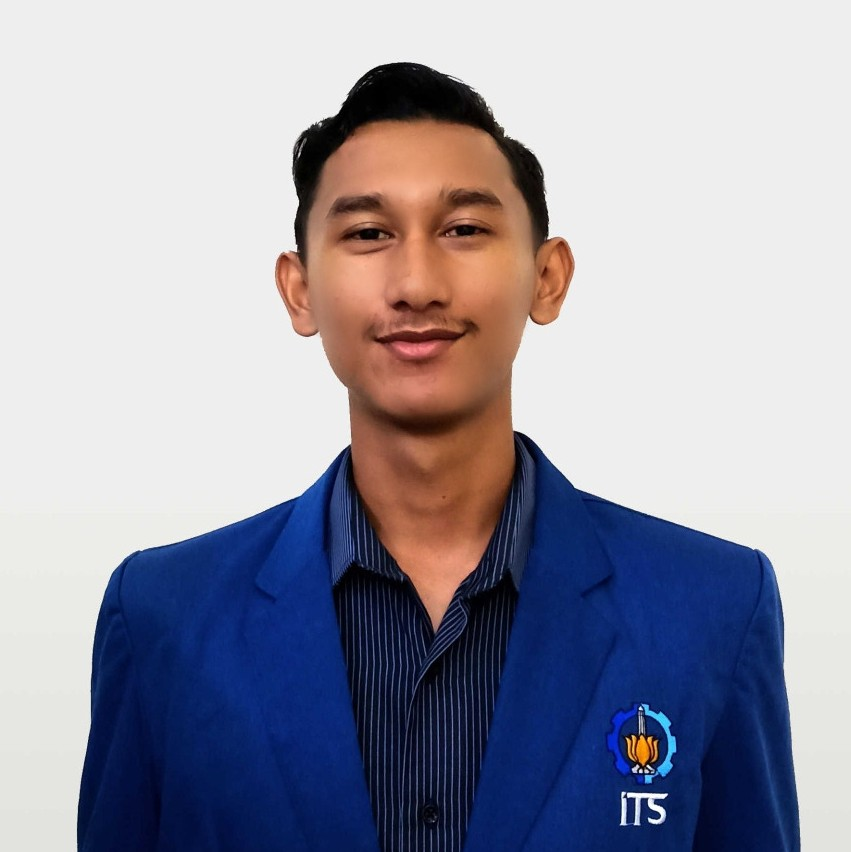
\includegraphics[width=0.3\textwidth]{images/roy.jpg}
  \vspace{-4ex}
\end{wrapfigure}

% Ubah kalimat berikut dengan biografi dari mahasiswa
Muhammad Roychan Meliaz, lahir pada 30 Mei 1999 di Kota Batam. Penulis telah menyelesaikan pendidikan formal di SDIT Darussalam 01 Batam (2005-2011), SMPN 03 Batam (2011-2014), dan SMAN 1 Batam (2014-2017). Pada tahun 2017 penulis melanjutkan studi S1 di Institut Teknologi Sepuluh Nopember (ITS) di Surabaya, dengan Departemen Teknik Komputer. Selama masa perkuliahan, penulis aktif mengikuti kegiatan organisasi dan kepanitiaan yang terdapat di kampus, seperti MAGE dan beberapa kegiatan lainnya. Penulis juga aktif sebagai asisten laboratorium di Lab B201 Telematika, serta menjadi bagian dari tim Kontes Robot ABU Indonesia (KRAI) ITS dan telah bertanding di Kontes Robot Indonesia. Di luar kampus, penulis juga aktif sebagai pengurus di Forum Daerah (Forda) Kerukunan Pelajar Mahasiswa Kepulauan Riau – Surabaya (KPMKR-Surabaya) yang menaungi para pelajar dan mahasiswa asal Provinsi Kepulauan Riau yang melanjutkan studi pendidikan di Kota Surabaya. Untuk mengubungi penulis, dapat melalui alamat email berikut roychan.meliaz@gmail.com. 


